The DEF compiler is based on the Tapir branch of LLVM, that provides fork-join parallelism primitives.\cite{TAPIR}\cite{LLVM}  The front-end is principly written in OCaml.  Likewise, the \texttt{defghi} utility is written in OCaml.\cite{DEF}

\subsection{Basic Syntax}

\begin{figure}[htbp!]
        \centering
        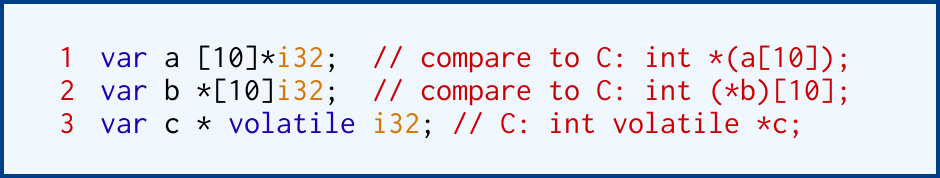
\includegraphics[scale=0.25]{gfx/types}
        \caption{Examples of variable declarations in DEF.  C allows the parentheses to be omitted in the first case, though they're provided to make precedence explicit.}
        \label{fig:types}
\end{figure}

Syntactically, DEF looks similar to C with the most apparent difference being that scopes are denoted by keywords instead of curly braces (e.g., \texttt{if} and \texttt{fi}, \texttt{do} and \texttt{od}, etc.) allowing curly braces to be repurposed for tuples.  Native types specify a bit width, so C's \texttt{int} on most systems corresponds to DEF's \texttt{i32}.  Types are also designed to read left-to-right, so the return type in a function declaration has been moved to the right using an arrow notation similar to ML-like languages or Go.  For more complicated types, fig.~\ref{fig:types} gives an example of left-to-rightness where no parentheses are needed to distinguish an array of pointers to integers (line 1) from a pointer to an array of 32-bit integers (line 2).

\begin{figure}[htbp!]
        \centering
        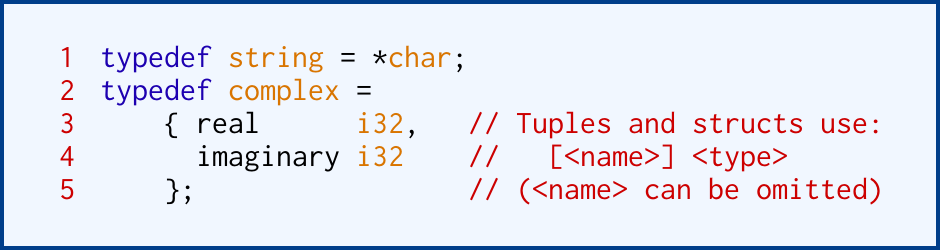
\includegraphics[scale=0.25]{gfx/typedef}
        \caption{Defining types with \texttt{typedef}.}
        \label{fig:typedef}
\end{figure}

Types are defined with the \texttt{typedef} keyword.  Figure \ref{fig:typedef} shows two examples: a C-style \texttt{string} type is defined on line 1, and a complex number struct is defined on lines 2-5.  The struct's actual definition is identical to tuple syntax, though tuples typically omit the member names.  Worthy of note is that tuples in DEF really are just anonymous structs, in keeping with the design goal of interchangeability with C.  Whereas in many languages tuples are allocated on the heap and garbage collected, in DEF they're allocated however a named struct would be in C.  Locating a struct or tuple on the heap requires explicit allocation.  Fig.~\ref{fig:window-find} provides a \texttt{window\_{}find} function declaration from the (FIXME: proper name and citation)Harris lock-free linked list in the Herlihy-Shavit book, as expressed in C (lines 2-6) and DEF (lines 9-10).  In both cases, the struct is returned by value on the stack.  A pointer, in both cases, would require explicit pointer syntax.

\begin{figure}[htbp!]
        \centering
        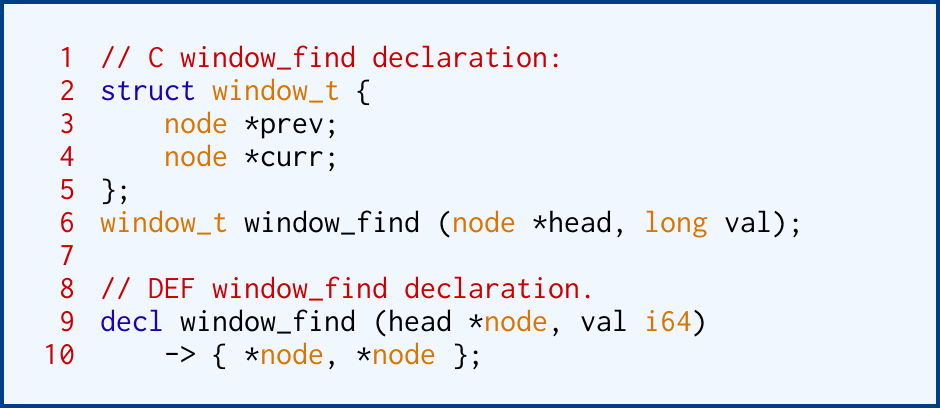
\includegraphics[scale=0.25]{gfx/window-find}
        \caption{Equivalent \texttt{window\_{}find} declarations in C and DEF.  The DEF tuple is an unnamed equivalent of C's \texttt{window\_{}t}.}
        \label{fig:window-find}
\end{figure}

\subsection{Allocation, Deallocation, and Reclamation}

DEF has no native allocator as distinct from C.  Allocating memory with \texttt{new} and deallocating it with \texttt{delete}, use \texttt{malloc} and \texttt{free}, respectively.  Since DEF's memory reclamation system is implemented using Forkscan, they implicitly use Forkscan's \texttt{malloc} and \texttt{free} wrappers, but the overhead of this indirection is undetectable in trials.  Independent of implementation, memory allocated with \texttt{new} is untracked.  Memory can be passed freely between DEF and C, and a pointer acquired in C through \texttt{malloc} can be deleted in DEF, and one acquired in DEF through \texttt{new} can be freed in C.

Moreover, \texttt{new} and \texttt{delete}, as applied to non-shared memory, are conveniences-only.  Mixing allocators or interfacing with a language with hooks to an external garbage collector is as trivial (or as complex) in DEF as it is in C because all memory is treated in exactly the same way.

The exception to this is in the use of \texttt{retire} to flag a pointer for tracking.  It's assumed that a retired node was allocated with \texttt{new}.  Implementation-wise, Forkscan requires knowledge of the \texttt{free} and \texttt{malloc\_{}usable\_{}size} corresponding to the \texttt{malloc} that was used to acquire the memory.  More broadly, it's hard to see how any implementation could call the correct \texttt{free} on a retired node unless it corresponded to the known \texttt{malloc}.
